\documentclass[12pt,a4paper]{article}

% --------------------
% Packages
% --------------------
\usepackage[top=2.5cm,bottom=2.5cm,left=2.7cm,right=2.7cm]{geometry}
\usepackage{amsmath,amssymb}
\usepackage{graphicx}
\usepackage{booktabs}
\usepackage{setspace}
\usepackage{indentfirst}
\usepackage{titlesec}
\usepackage{xcolor}
\usepackage{array}
\usepackage[T1]{fontenc}
\usepackage[utf8]{inputenc}
\usepackage{lmodern}
\usepackage[colorlinks=true,linkcolor=blue,citecolor=blue,urlcolor=blue]{hyperref}

% --------------------
% Layout settings
% --------------------
\setstretch{1.35}
\setlength{\parskip}{0.3em}
\setlength{\parindent}{1.2cm}

% --------------------
% Section formatting
% --------------------
\titleformat{\section}
{\Large\bfseries}
{\thesection}
{0.8em}
{}

\titleformat{\subsection}
{\large\bfseries}
{\thesubsection}
{0.8em}
{}

\begin{document}
	
	\begin{titlepage}
		\centering
		
		\vspace*{2cm}
		
		{\Huge\bfseries Technical Project Report\par}
		\vspace{0.6cm}
		
		{\LARGE\bfseries 
			\href{https://github.com/alitkbbl/PhysioStress}{\textcolor{blue}{PhysioStress}}
			\par}
		
		\vspace{0.5cm}
		{\large\itshape Technical Report\par}
		
		\vspace{0.8cm}
		\rule{\linewidth}{0.4pt}
		\vspace{0.8cm}
		
		{\Large Ali Taghizadeh\par}
		\vspace{0.3cm}
		
		{\large Faculty of Computer Science, Amirkabir University of Technology\par}
		
		\vfill
		
		\vspace*{1.5cm}
	\end{titlepage}
	
	\tableofcontents
	\newpage
	
	\section{Background}
	
	\subsection{Why do physiological signals reflect stress?}
	
	The autonomic nervous system (ANS) consists of two branches that continuously and involuntarily regulate the body: the \textbf{sympathetic} branch (``fight or flight,'' activated by threat or effort) and the \textbf{parasympathetic} branch (``rest and digest,'' dominant during calm states). Acute psychological stress triggers a sympathetic surge with detectable multisystem physiological signatures:
	
	\begin{itemize}
		\item \textbf{Increased heart rate and reduced heart rate variability (HRV):} A calm heart does not beat like a metronome; instead, it speeds up and slows down with each breath, a process largely controlled by the vagus nerve. Sympathetic activation suppresses this vagally mediated variability. Therefore, low HRV combined with elevated heart rate is one of the most reproducible markers of stress in the psychophysiology literature.
		
		\item \textbf{Increased skin conductance:} Sweat glands in the skin, especially on the palms, wrist, and fingers, are driven almost exclusively by sympathetic nerves, making electrodermal activity (EDA) one of the few peripheral signals with an almost direct relationship to sympathetic arousal. EDA has a slowly moving baseline level (the \textbf{tonic} component, or skin conductance level) and rapid discrete peaks (the \textbf{phasic} skin conductance responses, SCRs) synchronized with arousing events.
		
		\item \textbf{Breathing becomes faster and shallower:} Preparing the body for action increases the breathing rate while simultaneously reducing the depth of each breath.
		
		\item \textbf{Muscle contraction:} Body stiffening, jaw clenching, and general postural tension increase electromyographic (EMG) activity, especially in the upper body.
		
		\item \textbf{Reduced peripheral skin temperature:} Blood is redirected from the skin toward large muscles and the body core (vasoconstriction), producing the familiar sensation of ``cold hands.''
		
		\item \textbf{Changes in movement patterns:} Restlessness during stress and gesture- or laughter-related motion during amusement both differ from the relative stillness of the baseline resting state.
	\end{itemize}
	
	Because \textit{each of these signals} can be measured by wearable devices, and because amusement (a distinct high-arousal but positively valenced state) also perturbs several of them, the goal of this project is to determine whether a machine learning model can distinguish stress not only from a calm baseline state \textbf{but also} from a non-stress high-arousal state. This makes the problem a more realistic 3-class classification task.
	
	\subsection{Why is this difficult?}
	
	Two major factors make wearable stress detection difficult in practice, both of which are directly addressed in the design of this project:
	
	\begin{enumerate}
		\item \textbf{Inter-individual differences:} Resting heart rate, typical skin conductance level, and the extent to which a person's body reacts to stress (their ``reactivity'') vary substantially across individuals for reasons unrelated to their current stress level. A useful model must generalize to a \textit{new person} it has never seen before, rather than simply memorizing the 14 subjects used for training.
		
		\item \textbf{Overlap between stress and other high-arousal states:} Amusement and stress are physiologically similar in several respects; for example, both can elevate heart rate and movement. As a result, the genuinely difficult classification boundary is usually between stress and amusement, not between stress and calmness.
	\end{enumerate}
	
	\section{Data}
	
	The dataset consists of 15 subjects, each equipped with two wearable devices:
	
	\begin{itemize}
		\item \textbf{Chest sensor band:} Includes ECG, EDA, EMG, respiration, skin temperature, and a 3-axis accelerometer, all sampled at 100 Hz.
		\item \textbf{Wrist-worn sensor:} Includes blood volume pulse (BVP), EDA, skin temperature, and a 3-axis accelerometer, sampled at smartwatch-like rates (BVP at 64 Hz, EDA/temperature at 4 Hz, and accelerometer at 32 Hz).
	\end{itemize}
	
	Data recording for each subject was performed under three conditions --- baseline (calm), stress, and amusement. The raw signals were generated using a physiology-informed synthetic model (\texttt{src/synthetic\_data.py}) designed so that each condition changes in the \textit{direction} expected from real autonomic physiology: higher heart rate and lower HRV under stress, increased EDA under stress, faster and shallower breathing under stress, stress-induced temperature drops caused by vasoconstriction, and so forth.
	
	\vspace{0.5cm}
	\noindent\textbf{Design goals for a realistic classification problem.} Two aspects of the signal-generation model are especially important for making the final classification task meaningful:
	
	\begin{enumerate}
		\item \textbf{Within-condition physiological drift:} Each driving parameter (instantaneous heart rate, HRV, and so on) evolves over the course of each multi-minute state segment according to a mean-reverting process, rather than remaining a fixed number throughout the interval.
		
		\item \textbf{Subject-specific reactivity:} Each subject is assigned a random subject-specific \textit{reactivity} for each signal, representing how much that signal shifts under stress independently of baseline level.
	\end{enumerate}
	
	The signals were segmented into 60-second windows with 50\% overlap, resulting in a total of \textbf{495 windows from 15 subjects}: 225 baseline, 165 stress, and 105 amusement.
	
	\begin{figure}[htbp]
		\centering
		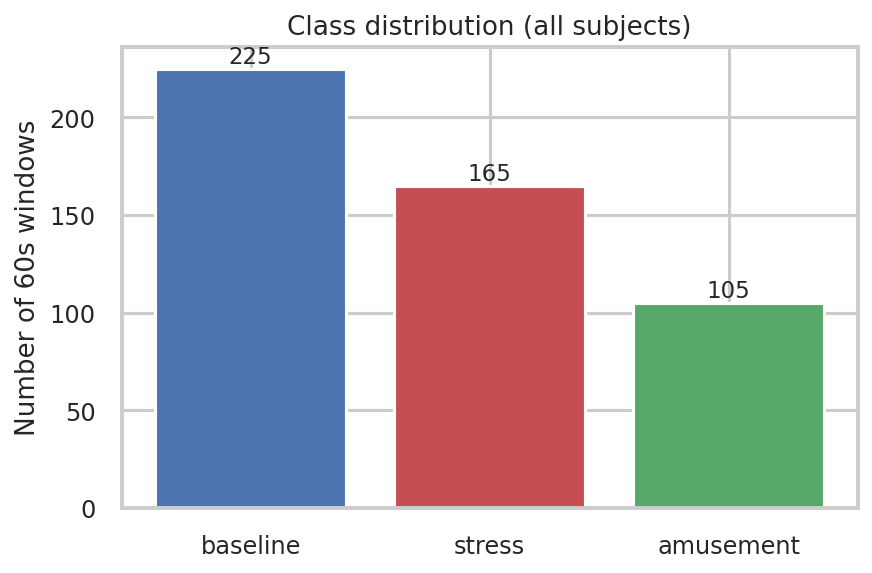
\includegraphics[width=0.7\textwidth]{../results/figures/class_distribution.png}
		\caption{Class distribution}
	\end{figure}
	
	\newpage
	\section{Methodology}
	
	\subsection{Analysis of extracted features and their physiological basis}
	
	To understand changes in physiological and psychological states such as stress and arousal, a variety of features are extracted from biosignals. This section provides a detailed discussion of each signal group, the key extracted features, and the physiological mechanisms behind them.
	
	\paragraph{1. Electrodermal activity (EDA, recorded from chest and wrist):}
	EDA is one of the most sensitive indicators of sympathetic nervous system (SNS) activity. The extracted features from this signal are mainly divided into two categories:
	\begin{itemize}
		\item \textbf{Tonic features:} These include the mean and slope of the tonic activity, representing long-term and gradual changes in skin conductance.
		\item \textbf{Phasic features:} These include the standard deviation of the phasic component, reflecting sudden short-term changes triggered by stimuli.
	\end{itemize}
	\textbf{Physiological interpretation:} Activation of the sympathetic nervous system in response to stress or emotional arousal increases secretion from eccrine sweat glands in the skin. This process increases the number of conductive pathways, lowers skin resistance, and raises conductance. An increase in general conductance level (tonic) together with more frequent and larger rapid electrodermal responses (phasic) provides a direct indicator of sympathetic arousal.
	
	\paragraph{2. Heart rate variability (HRV):}
	HRV reflects the interaction between the sympathetic and parasympathetic (vagal) branches of the autonomic nervous system. The extracted indices include:
	\begin{itemize}
		\item \textbf{Time-domain indices:} Mean heart rate (HR), standard deviation of beat intervals (SDNN), and root mean square of successive differences (RMSSD).
		\item \textbf{Frequency-domain indices:} The low-frequency to high-frequency power ratio (LF/HF).
	\end{itemize}
	\textbf{Physiological interpretation:} During calm states, vagal activity is high and exerts a braking effect on the sinoatrial node, leading to larger fluctuations in beat intervals (high HRV). Under stress and psychological pressure, vagal regulation decreases and sympathetic pathways become dominant. This makes beat intervals more uniform and leads to a meaningful reduction in SDNN and RMSSD. An increase in the LF/HF ratio is commonly interpreted as a shift in sympathovagal balance toward sympathetic dominance.
	
	\paragraph{3. Electromyography (EMG):}
	EMG measures the electrical activity of muscles. Key extracted statistical and frequency-related indices include root mean square (RMS), signal amplitude standard deviation, and zero-crossing rate (ZC).  
	\textbf{Physiological interpretation:} Under stress, the body unconsciously enters a ``fight-or-flight'' state. This defensive response is accompanied by contraction of voluntary and involuntary muscles, especially in the shoulders, neck, and face, to prepare the body for physical action. Increased RMS reflects greater recruitment of motor units and higher firing rates due to tension.
	
	\paragraph{4. Respiratory tension and breathing patterns:}
	Extracted features include respiration rate (breaths per minute), inhalation and exhalation amplitude, and variability in respiration rate.  
	\textbf{Physiological interpretation:} The respiratory system is strongly affected by both metabolic demand and emotional state. Under stress, sympathetic stimulation causes bronchodilation and increases the breathing rate to accelerate oxygen delivery to tissues. This process usually results in faster, shallower breathing (reduced effective amplitude) and more irregular respiratory patterns.
	
	\paragraph{5. Skin temperature:}
	Features extracted from temperature sensors include mean temperature, the slope of temperature change over time, and temperature standard deviation.  
	\textbf{Physiological interpretation:} The physiological stress response includes redistribution of blood flow from peripheral areas (skin and extremities such as fingers) toward vital organs and large muscles. This process, driven by sympathetic alpha-adrenergic vasoconstriction, causes a noticeable drop in peripheral skin temperature and changes in temperature slope.
	
	\paragraph{6. Accelerometer:}
	Extracted features include the mean and standard deviation of total acceleration magnitude across the three axes, as well as movement energy.  
	\textbf{Physiological interpretation:} Accelerometer data are useful not only for filtering motion artifacts in other signals (such as removing movement-induced noise from EDA and HRV), but also for revealing behavioral patterns associated with stress. For example, restless movement, mild hand tremor, or stress-related freezing and rigid focus generate distinct energy and variability patterns in the accelerometer signal, which help distinguish cognitive and affective states.
	
	\newpage
	\section{Results}
	
	\subsection{Model Comparison}
	
	\begin{table}[htbp]
		\centering
		\begin{tabular}{lccc}
			\toprule
			\textbf{Model} & \textbf{Accuracy} & \textbf{Macro F1-Score} & \textbf{LOSO Accuracy Std} \\
			\midrule
			\textbf{Gradient Boosting (HistGB)} & \textbf{0.891} & \textbf{0.862} & 0.067 \\
			Random Forest & 0.875 & 0.839 & 0.096 \\
			Logistic Regression & 0.853 & 0.810 & 0.097 \\
			SVM (RBF) & 0.804 & 0.745 & 0.110 \\
			Baseline (Majority Class) & 0.455 & 0.208 & 0.000 \\
			\bottomrule
		\end{tabular}
		\caption{Performance comparison of various models across 15 subjects.}
	\end{table}
	
	\begin{figure}[htbp]
		\centering
		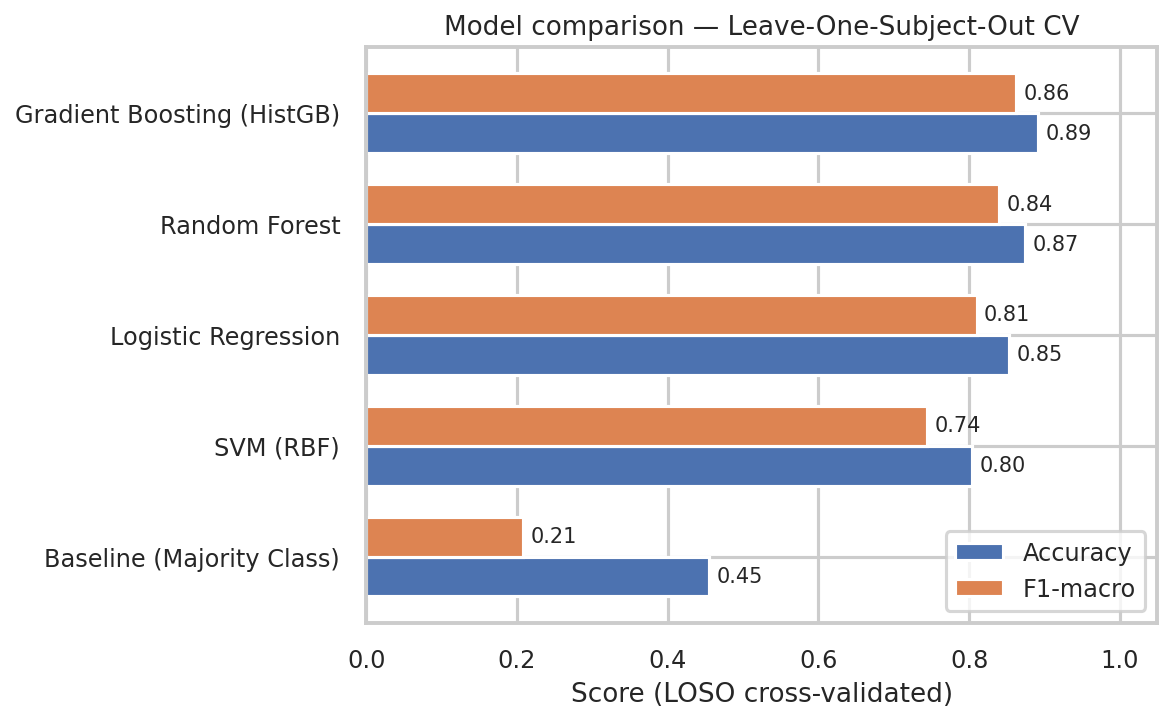
\includegraphics[width=0.8\textwidth]{../results/figures/model_comparison.png}
		\caption{Model comparison}
	\end{figure}
	
	All real models perform substantially better than the baseline. Tree-based methods (gradient boosting and random forest) outperform linear and kernel-based methods, suggesting that the relationship between the features and the target classes is nonlinear and threshold-like. For example, movement-related features may remain near zero during rest and then increase abruptly once motion begins.
	
	\subsection{Confusion Matrix (Best Model, aggregated across all 15 LOSO folds)}
	
	\begin{figure}[htbp]
		\centering
		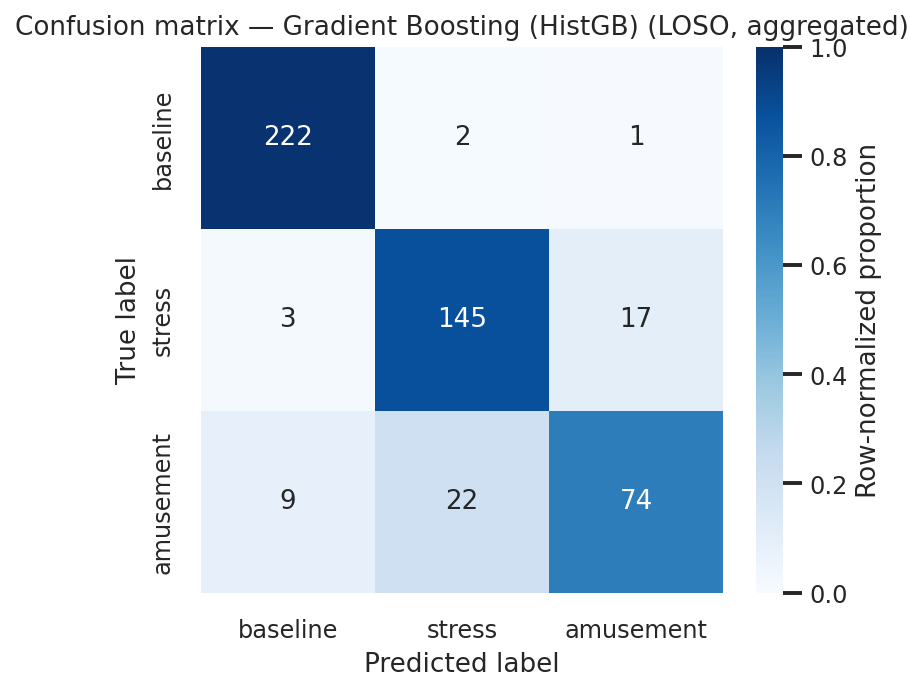
\includegraphics[width=0.7\textwidth]{../results/figures/confusion_matrix_best_model.png}
		\caption{Confusion matrix of the best model}
	\end{figure}
	
	\textbf{The baseline state is classified almost perfectly} (222 out of 225, corresponding to 98.7\% recall). Physiologically, this is the ``quietest'' condition and therefore the easiest to separate. The dominant classification error is \textbf{confusion between stress and amusement} (17 stress samples predicted as amusement and 22 amusement samples predicted as stress). This is exactly what physiology would predict: both states involve high sympathetic arousal, and the boundary between them is inherently the hardest one to separate.
	
	\subsection{Between-subject LOSO variance}
	
	The best model (gradient boosting) shows meaningful differences in accuracy across held-out individuals:
	
	\begin{figure}[htbp]
		\centering
		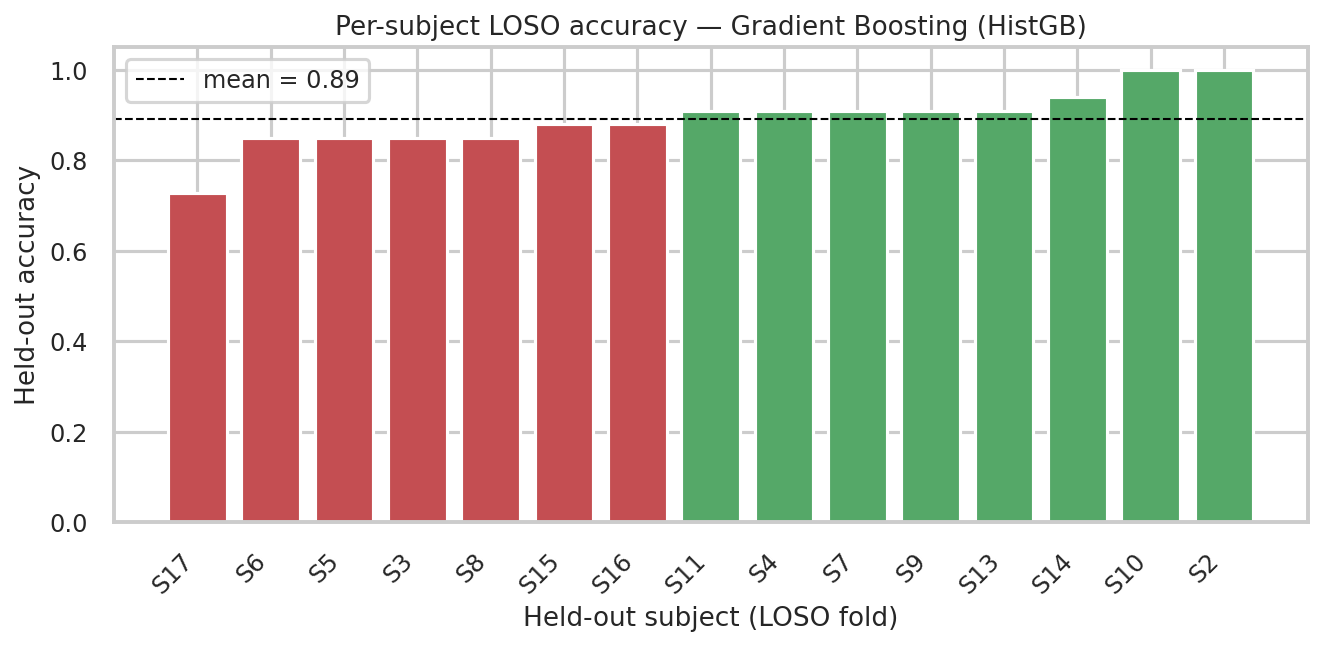
\includegraphics[width=0.8\textwidth]{../results/figures/loso_per_subject_accuracy.png}
		\caption{Per-subject model accuracy (LOSO)}
	\end{figure}
	
	Subject \texttt{S17}, the hardest case, achieved an accuracy of 0.727, several subjects fell between 0.848 and 0.939, and subjects \texttt{S2} and \texttt{S10} were classified perfectly at 1.000. The overall mean is 0.891 with a standard deviation of 0.067, indicating real dispersion and showing that \textbf{generalization to new individuals is much more difficult for some subjects than for others}.
	
	\subsection{Independent replication and normalization-ablation analysis (Notebook 03)}
	
	An independent implementation in \texttt{Notebook 03} tested whether per-subject baseline normalization was actually beneficial, or whether a standard global scaler (\texttt{StandardScaler}) was sufficient. The results showed:
	
	\begin{itemize}
		\item Per-subject normalized model: accuracy = 0.891
		\item Global standardized model: \textbf{accuracy = 0.958}
	\end{itemize}
	
	\begin{figure}[htbp]
		\centering
		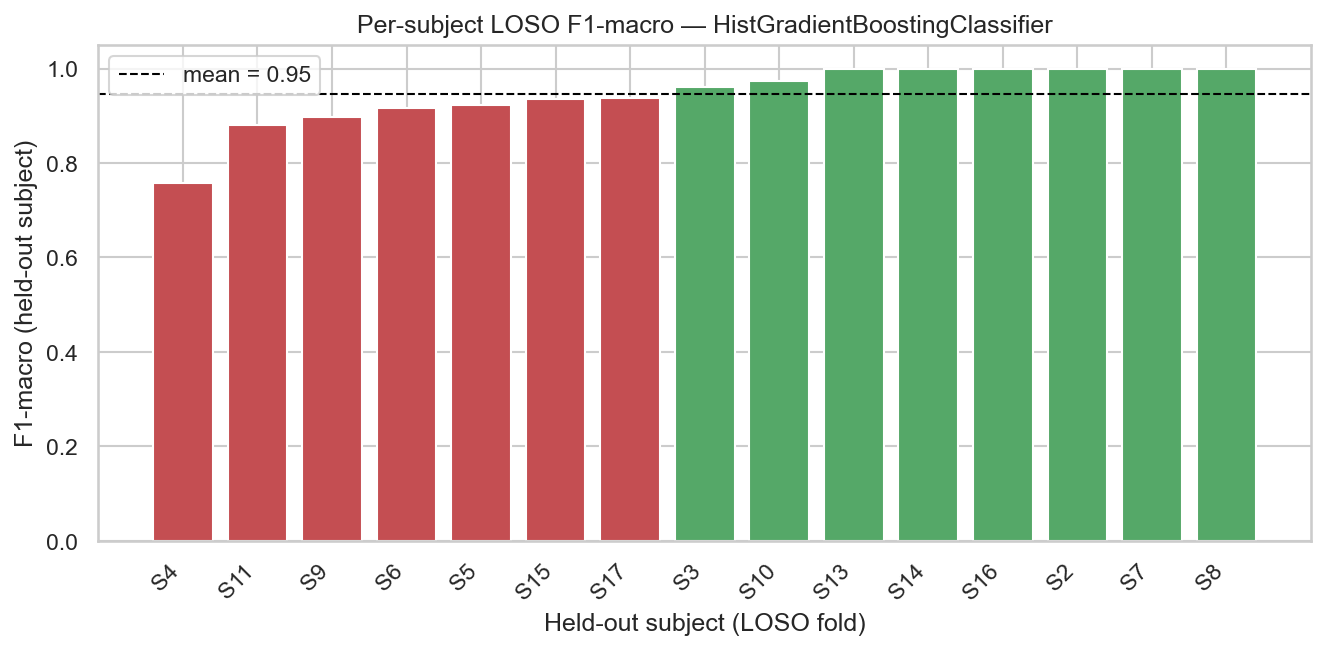
\includegraphics[width=0.48\textwidth]{../results/figures/loso_per_subject_f1.png}
		\hfill
		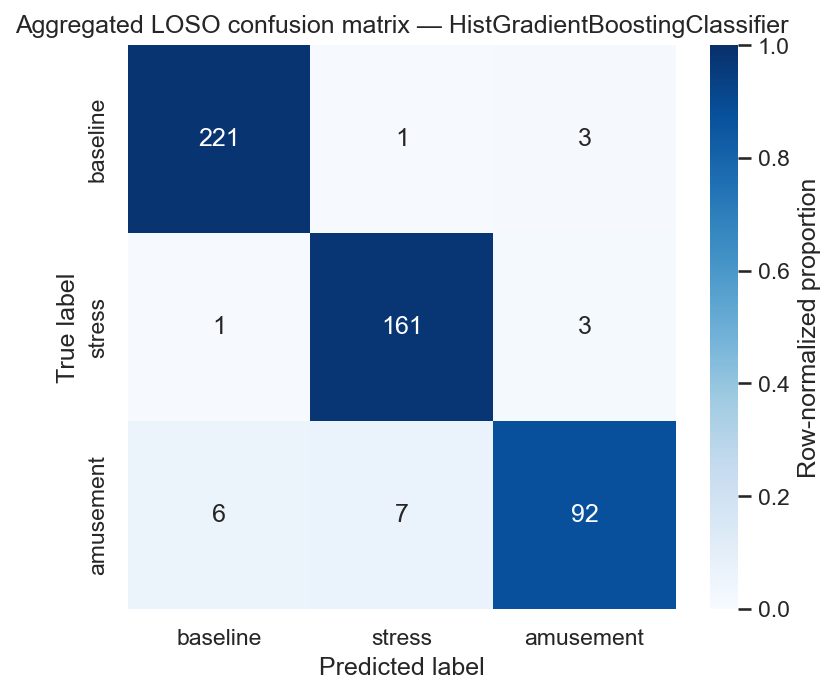
\includegraphics[width=0.48\textwidth]{../results/figures/loso_confusion_matrix.png}
		\caption{Per-subject F1-score and confusion matrix (Notebook 03)}
	\end{figure}
	
	The reason is that each subject's baseline features are estimated from only a small number of samples (roughly 15 windows), and the noise in that estimate outweighs the benefits of removing inter-individual differences. This is an important finding: \textbf{the normalization strategy is itself a modeling choice and must be evaluated empirically.}
	
	\newpage
	\section{Interpretability}
	
	Feature importance was computed using three independent methods:
	
	\begin{enumerate}
		\item \textbf{Permutation importance:} Computed on the held-out test subjects and averaged across all LOSO folds.
		\item \textbf{Shapley values:} A custom implementation from first principles using a sampling-based algorithm.
		\item \textbf{One-way ANOVA F-statistic:} A model-agnostic independent check.
	\end{enumerate}
	
	\subsection{Top features and contribution of each modality}
	
	\begin{figure}[htbp]
		\centering
		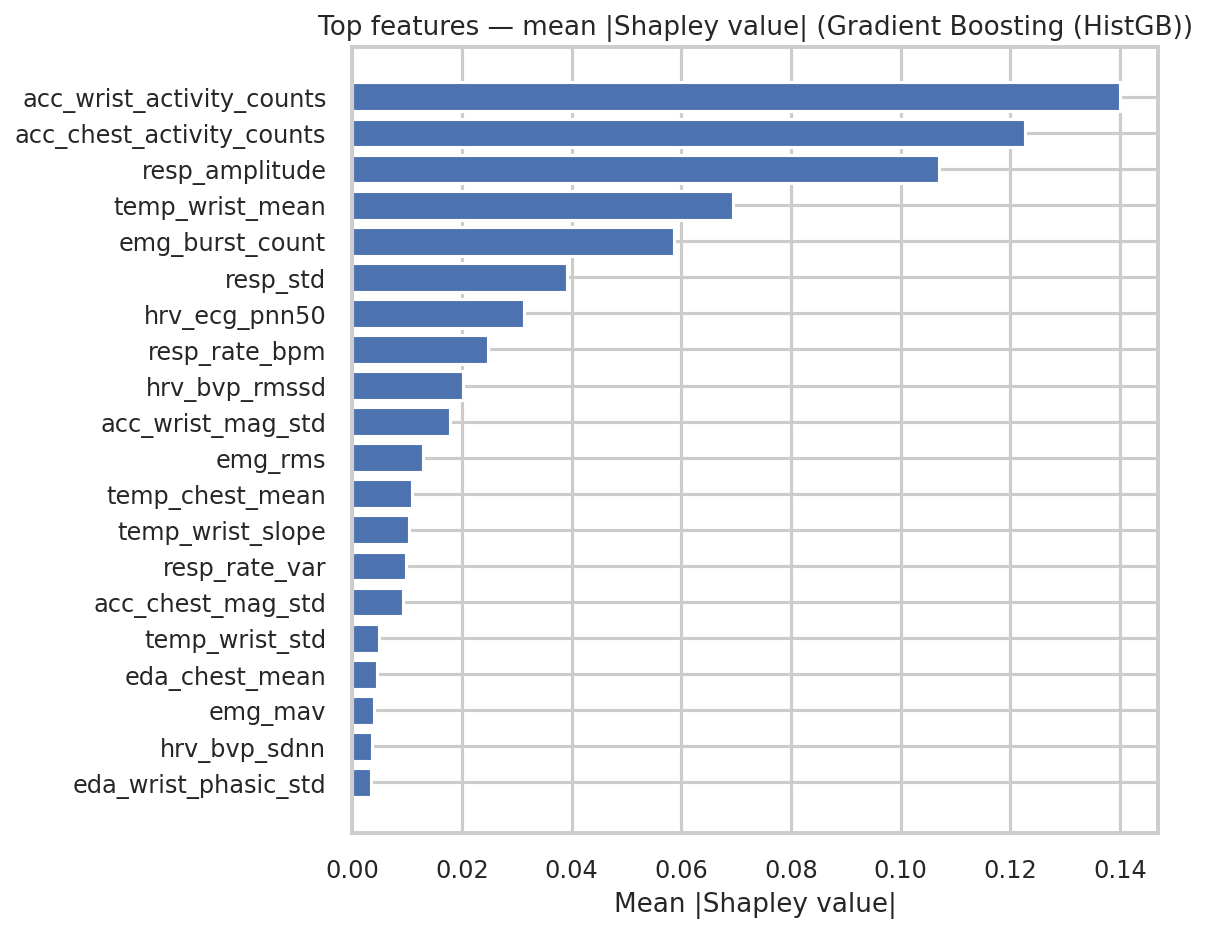
\includegraphics[width=0.8\textwidth]{../results/figures/feature_importance_shap.png}
		\caption{Feature importance based on SHAP values}
	\end{figure}
	
	\begin{figure}[htbp]
		\centering
		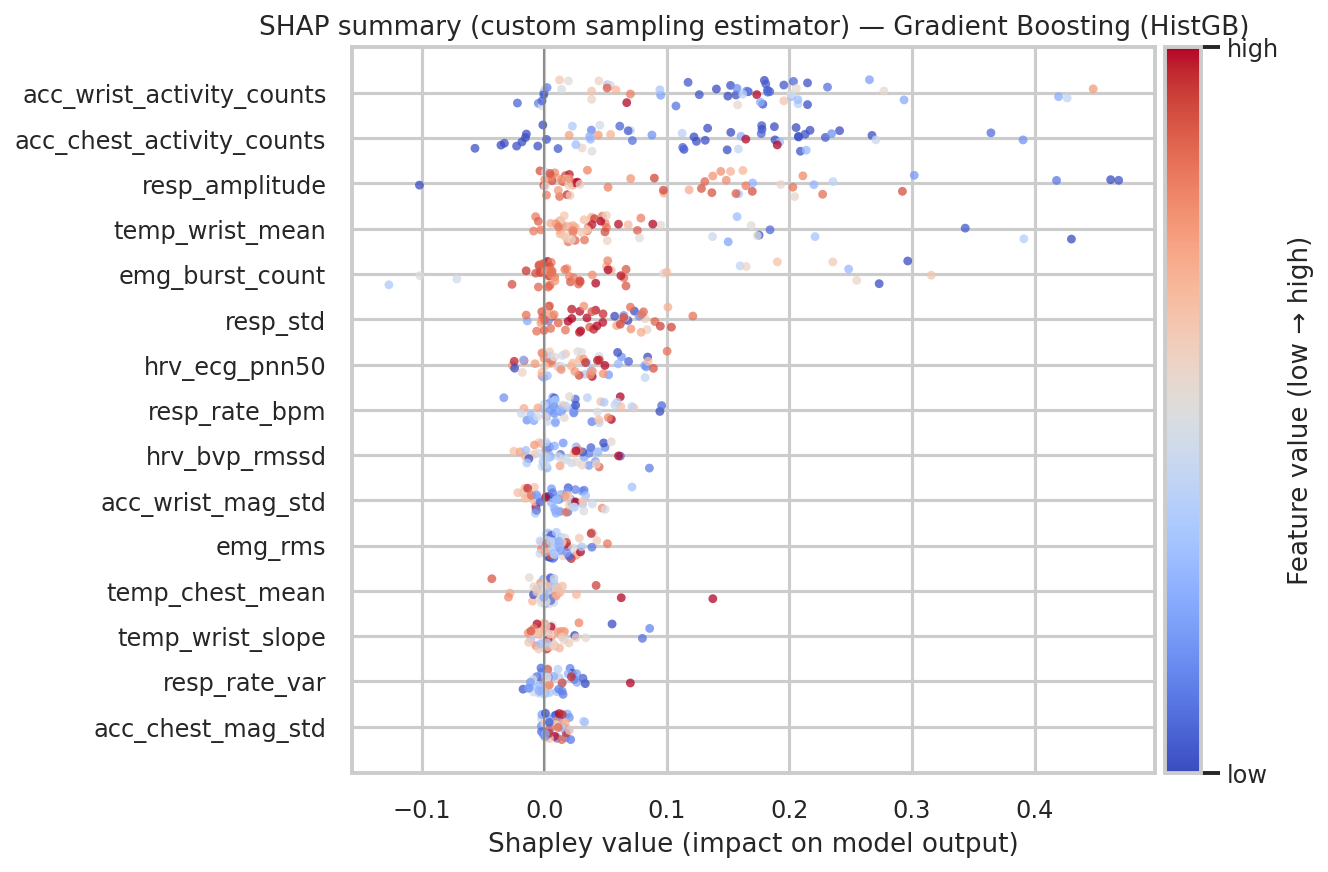
\includegraphics[width=0.8\textwidth]{../results/figures/shap_summary_beeswarm.png}
		\caption{SHAP beeswarm summary plot}
	\end{figure}
	
	\begin{figure}[htbp]
		\centering
		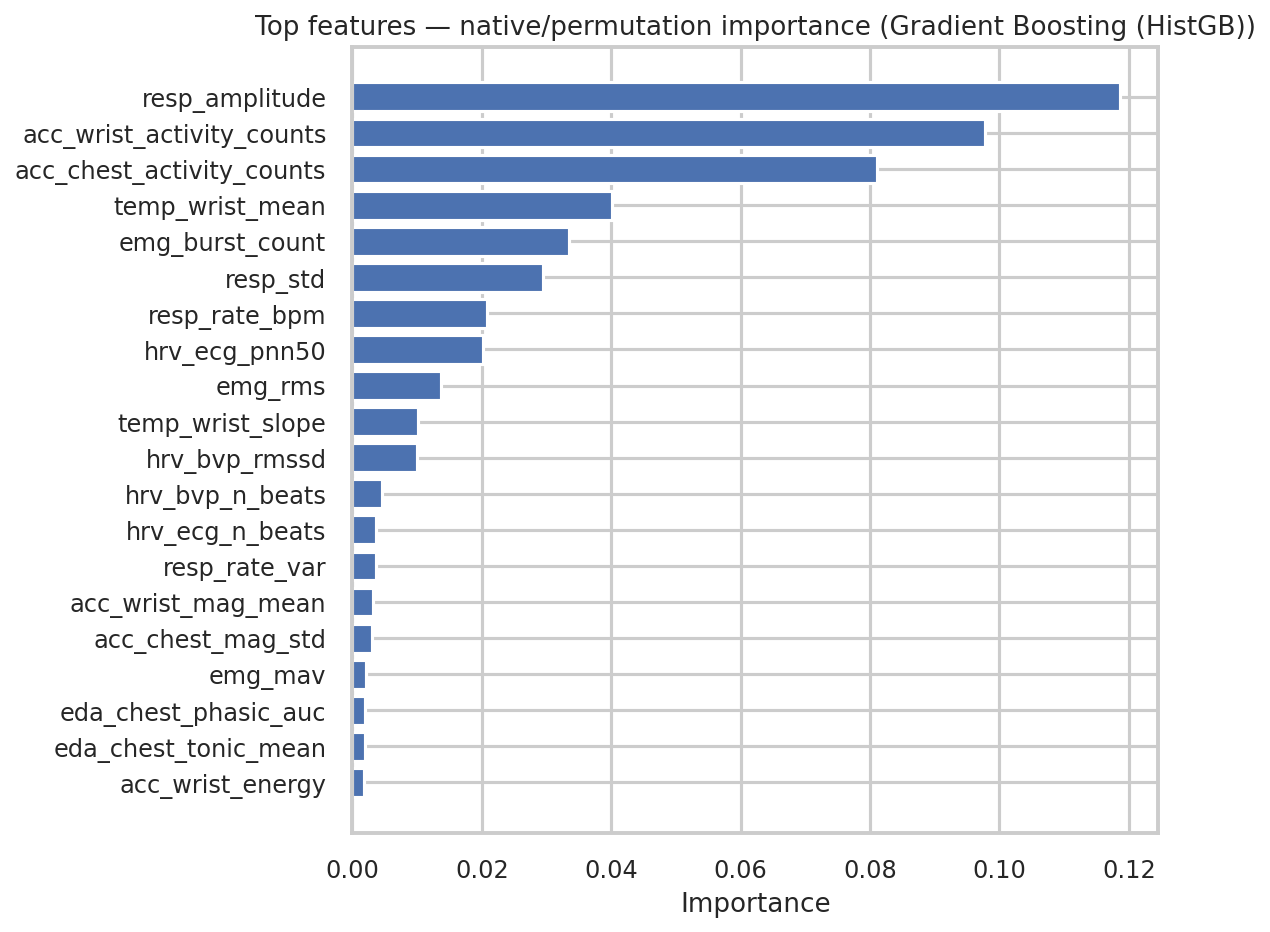
\includegraphics[width=0.8\textwidth]{../results/figures/feature_importance_native.png}
		\caption{Feature importance based on permutation importance}
	\end{figure}
	
	Both SHAP and permutation-based methods agree on the top five features.
	
	\subsection{Contribution of each signal modality}
	
	\begin{figure}[htbp]
		\centering
		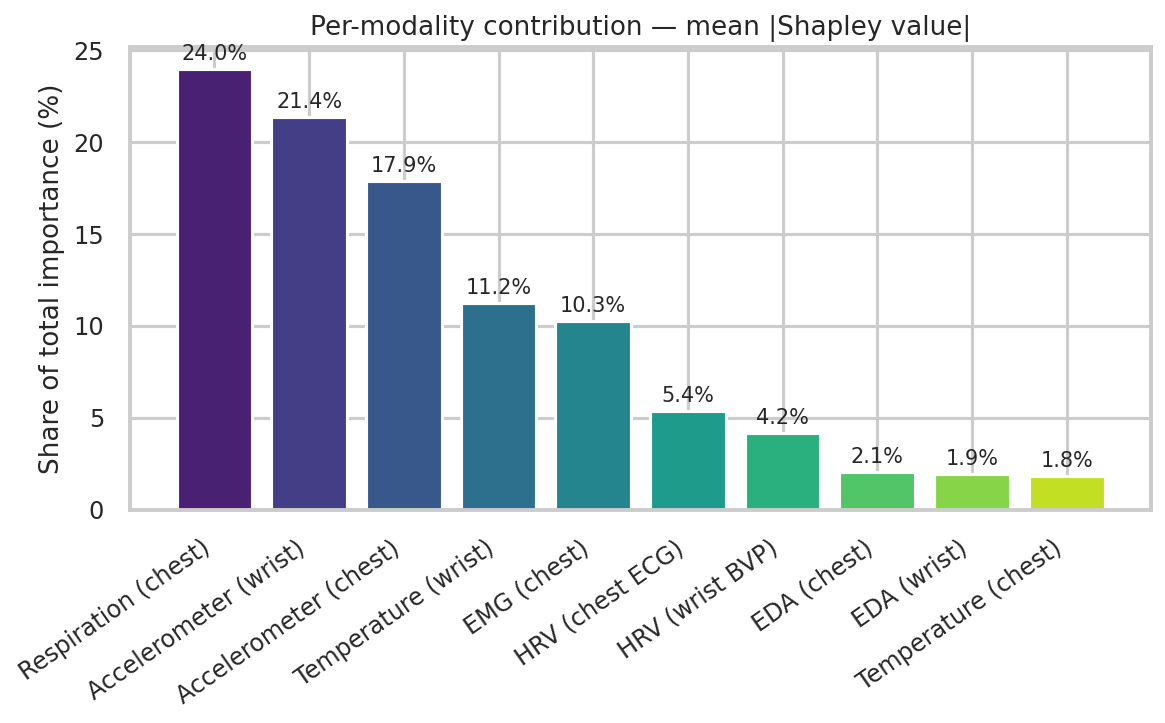
\includegraphics[width=0.8\textwidth]{../results/figures/modality_importance_shap.png}
		\caption{Modality importance based on SHAP}
	\end{figure}
	
	\begin{figure}[htbp]
		\centering
		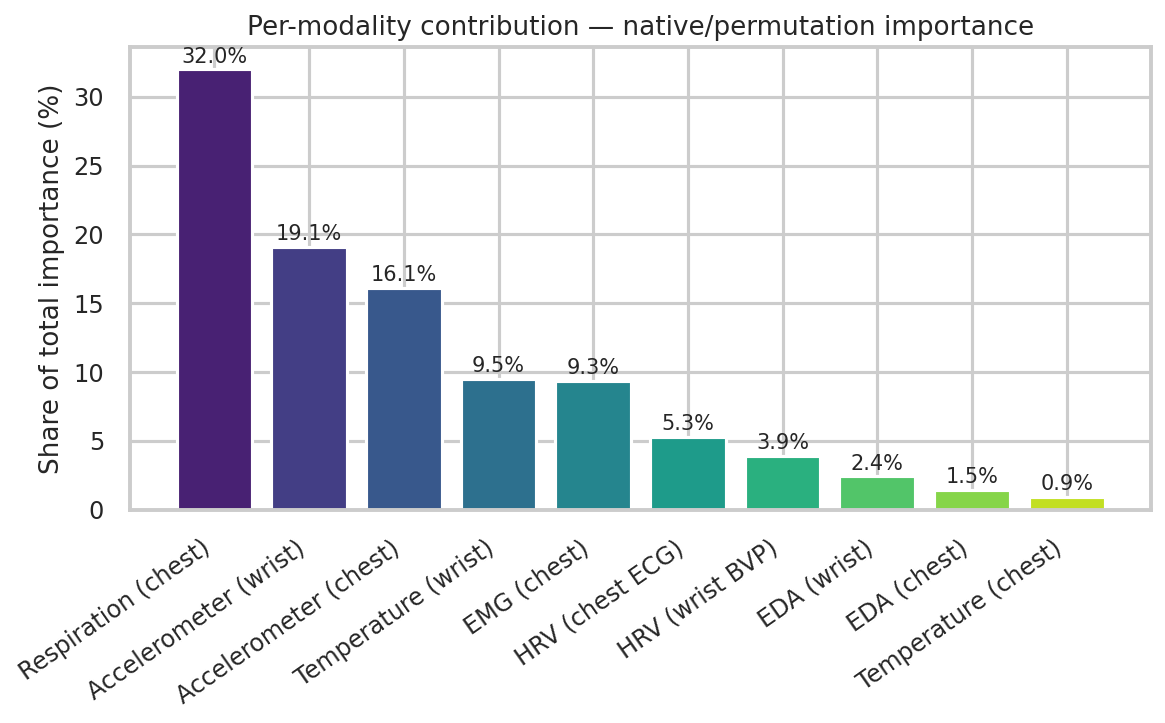
\includegraphics[width=0.8\textwidth]{../results/figures/modality_importance_native.png}
		\caption{Modality importance based on permutation importance}
	\end{figure}
	
	\begin{figure}[htbp]
		\centering
		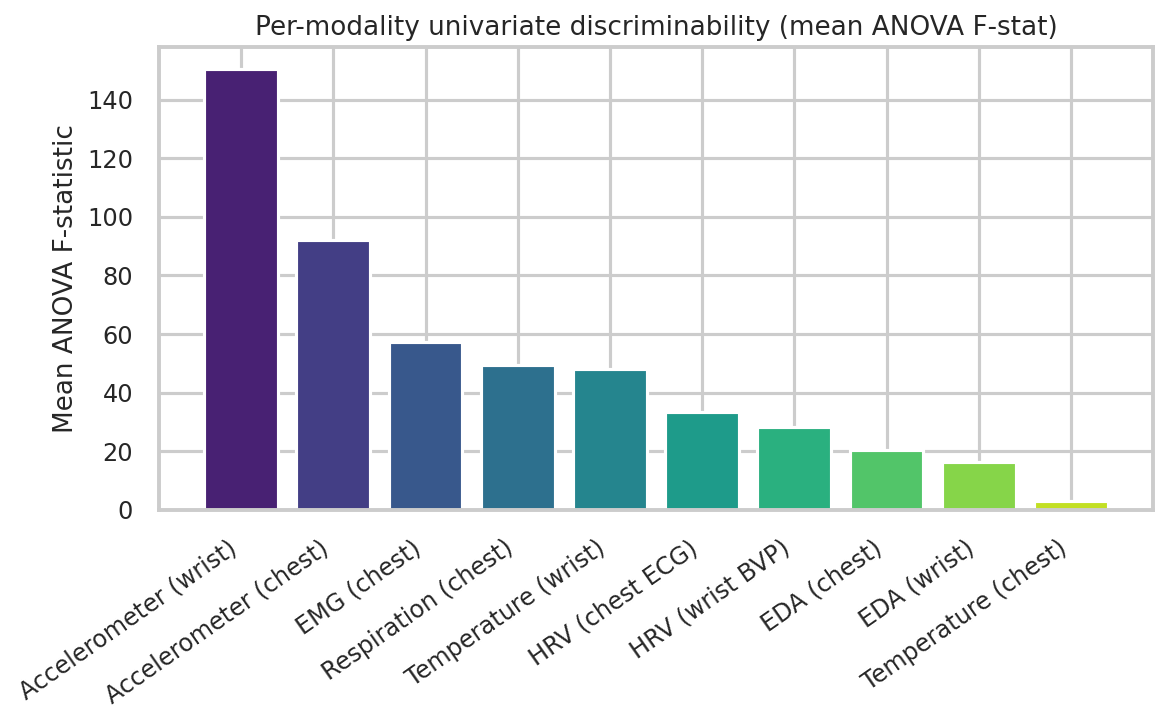
\includegraphics[width=0.8\textwidth]{../results/figures/modality_importance_univariate.png}
		\caption{Modality importance based on the univariate method}
	\end{figure}
	
	\textbf{Plain-language interpretation:} Respiration and movement dominate. Rapid, shallow breathing is among the fastest signs of sympathetic activation. Accelerometer activity is also highly informative because the body tends to become restless under stress, laughs and moves more during amusement, and remains relatively still during baseline. Reduced wrist temperature and increased muscle contraction are also classic indicators of stress.
	
	\textbf{Why is EDA not at the very top?} First, because of redundancy in the data: once the model learns changes in respiration and movement, the additional information provided by EDA becomes more marginal. Second, this result is specific to the feature set defined in this project.
	
	\newpage
	\section{Discussion}
	
	\subsection{What worked well}
	
	\begin{itemize}
		\item The LOSO protocol together with the normalization strategies produced a model that generalizes well to unseen individuals (accuracy 0.891 versus baseline 0.455).
		\item All three interpretability methods agreed on a shared set of top features.
		\item The independent implementation confirmed that respiration and movement are the dominant modalities.
	\end{itemize}
	
	\subsection{What was less successful and error analysis}
	
	\begin{itemize}
		\item \textbf{The stress-amusement boundary remains difficult:} Of the 44 total classification errors, 39 occurred between these two classes. Distinguishing these two high-arousal states likely requires sensitivity to \textit{affective valence}, which peripheral physiological signals capture only weakly.
		\item \textbf{Variation in subject-level generalization:} The drop in accuracy for some subjects (such as \texttt{S17}) likely reflects lower-than-average physical reactivity to stress in modalities such as respiration and muscle activity.
	\end{itemize}
	
	\section{References}
	
	\begin{itemize}
		\item Štrumbelj, E., \& Kononenko, I. (2010). An Efficient Explanation of Individual Classifications using Game Theory. \textit{Journal of Machine Learning Research}, 11, 1--18.
		\item Lundberg, S. M., \& Lee, S.-I. (2017). A Unified Approach to Interpreting Model Predictions. \textit{Advances in Neural Information Processing Systems} (NeurIPS 2017).
		\item Pedregosa, F., et al. (2011). Scikit-learn: Machine Learning in Python. \textit{Journal of Machine Learning Research}, 12, 2825--2830.
		\item Virtanen, P., et al. (2020). SciPy 1.0: Fundamental Algorithms for Scientific Computing in Python. \textit{Nature Methods}, 17, 261--272.
	\end{itemize}
	
\end{document}
